\chapter{METODOLOGÍA DE LA INVESTIGACIÓN}

\section{Diseño de la investigación}
La metodología de investigación es fundamental para asegurar que los objetivos del estudio se alcancen de manera eficiente y rigurosa. En este capítulo se detallan los pasos y procedimientos que se seguirán para llevar a cabo la investigación sobre la implementación de un chatbot médico pediátrico para servicios en áreas rurales del Perú. Este diseño permitirá una evaluación exhaustiva de la viabilidad, usabilidad y efectividad del chatbot en mejorar el acceso a servicios de salud pediátrica en contextos rurales.

\subsection{Tipo de Investigación}
La presente investigación se clasifica como una investigación aplicada con un enfoque cuantitativo y cualitativo (mixto). El objetivo es diseñar, implementar y evaluar la efectividad de un chatbot médico pediátrico para servicios en áreas rurales del Perú. La combinación de ambos enfoques permite una comprensión integral del problema y la evaluación de la solución propuesta.

\subsection{Enfoque de Investigación}
El enfoque de la investigación es exploratorio-descriptivo. Exploratorio porque se busca investigar un área poco estudiada y obtener una comprensión inicial del uso de chatbots en la atención médica pediátrica en zonas rurales. Descriptivo porque se pretende detallar y analizar el funcionamiento del chatbot y su impacto en la población objetivo.

\section{Población y Muestra}
\begin{table}[H]
	\centering
	\begin{tabular}{|>{\raggedright\arraybackslash}p{4cm}|>{\raggedright\arraybackslash}p{10cm}|}
		\hline
		\textbf{Población} & Preguntas y respuestas entre Doctores y Pacientes \\ \hline
		\textbf{Muestra} & Se seleccionará una muestra de las conversaciones sobre las preguntas y respuestas relacionados a niños menores de 12 años. \\ \hline
		\textbf{Unidad de análisis} & Conversaciones sobre las preguntas y respuestas relacionados a niños menores de 12 años y los profesionales de salud. \\ \hline
		\textbf{Variable y tipo de análisis} & Satisfacción del usuario (Cuantitativo) - Eficiencia del chatbot (Cuantitativo) - Opiniones y experiencias de uso (Cualitativo). \\ \hline
	\end{tabular}
	\caption{Descripción de la población de estudio}
	\label{tab:descripcion_poblacion}
\end{table}

\section{Operacionalización de Variables}
\begin{table}[H]
	\centering
	\caption{Operacionalización de Variables}
	\begin{tabular}{|p{2cm}|p{3cm}|p{3cm}|p{2cm}|p{4cm}|}
		\hline
		\textbf{Variable} & \textbf{Definición Operacional} & \textbf{Indicador} & \textbf{Tipo de Variable} & \textbf{Fórmula} \\ \hline
		Satisfacción del usuario & Nivel de satisfacción de los pacientes y cuidadores con el uso del chatbot & Puntuación en encuestas de satisfacción & Cuantitativa & \(\text{\tiny Satisfacción} = \frac{\sum \text{\tiny Puntuaciones}}{\text{\tiny Número de respuestas}}\) \\ \hline
		Eficiencia del chatbot & Capacidad del chatbot para resolver consultas médicas & Tiempo de respuesta y precisión & Cuantitativa & \(\text{Eficiencia} = \frac{\text{\tiny Consultas resueltas}}{\text{\tiny Total de consultas}} \times 100\%\) \\ \hline
		Opiniones y experiencias & Percepciones y comentarios de los usuarios sobre el chatbot & Testimonios y entrevistas & Cualitativa & N/A \\ \hline
	\end{tabular}
\end{table}



\section{Técnicas de recolección}
\begin{itemize}
	\item Base de datos: Conjunto de Preguntas (Paciente) y Respuestas (Doctor)
	\item Encuestas: Para medir la satisfacción de los usuarios y la eficiencia del chatbot.
	\item Entrevistas: Para recoger opiniones y experiencias detalladas de los usuarios.
	\item Registros del sistema: Para analizar la precisión y tiempo de respuesta del chatbot.
	
\end{itemize}


\section{Técnicas para el Procesamiento y Análisis de la Información}

\subsection{Metodología de la Implementación de la Solución}

\begin{figure}[H]
	\begin{center}
		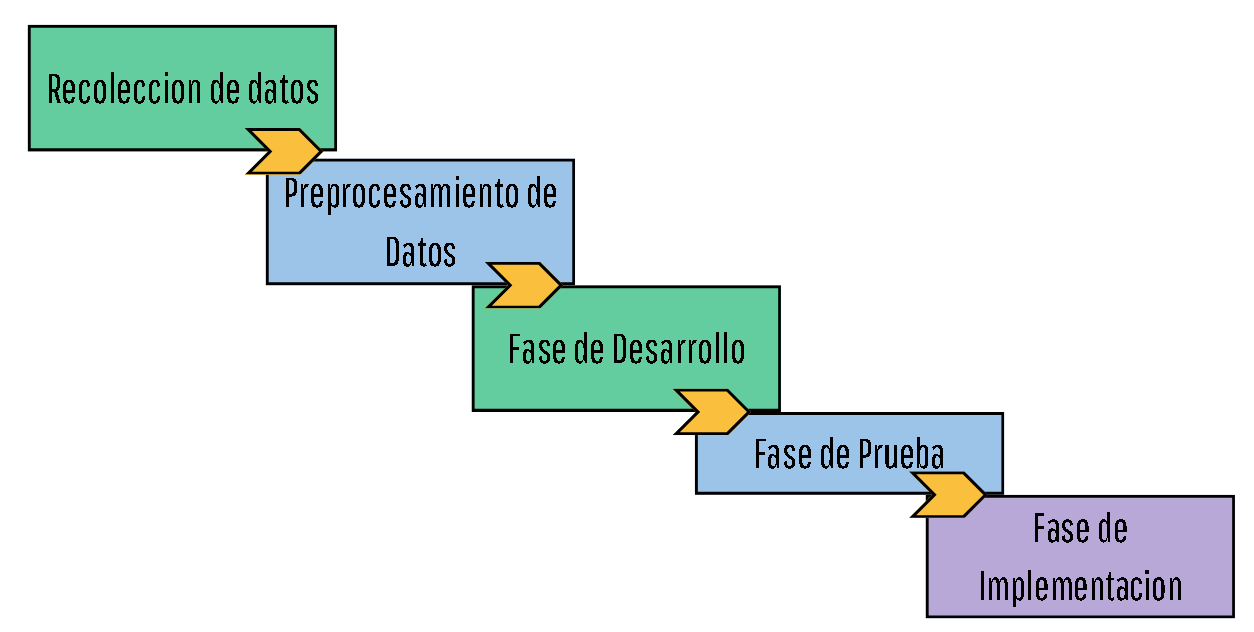
\includegraphics[width=0.6\textwidth]{images_repo/METOD_CHATBOT_JP.png}
		\caption{Metodologia, Fuente: Propio}
		\label{1:fig}
	\end{center}
\end{figure}
\vspace{5mm}
\begin{enumerate}
	\item \textbf{Fase de Desarrollo:}
	\begin{itemize}
		\item \textbf{Análisis de Requisitos:} Recolección de información detallada sobre las necesidades de los usuarios y los requerimientos funcionales y no funcionales del chatbot.
		\item \textbf{Diseño del Sistema:} Elaboración de diagramas de flujo, diseño de la arquitectura del sistema y definición de la base de datos.
		\item \textbf{Programación:} Implementación del chatbot utilizando tecnologías como Python, TensorFlow, y herramientas de procesamiento de lenguaje natural (NLP) como spaCy o NLTK.
		\item \textbf{Pruebas Unitarias:} Realización de pruebas en cada módulo del chatbot para asegurar su correcto funcionamiento individual.
	\end{itemize}
	
	\item \textbf{Fase de Prueba:}
	\begin{itemize}
		\item \textbf{Pruebas Piloto:} Implementación del chatbot en un entorno controlado con un grupo pequeño de usuarios para identificar problemas y áreas de mejora.
		\item \textbf{Recopilación de Feedback:} Recolección de opiniones y sugerencias de los usuarios que participaron en la prueba piloto.
		\item \textbf{Mejoras y Ajustes:} Modificaciones en el chatbot basadas en el feedback recibido durante las pruebas piloto.
	\end{itemize}
	
	\item \textbf{Fase de Implementación:}
	\begin{itemize}
		\item \textbf{Despliegue:} Instalación y configuración del chatbot en la plataforma final para su uso por la población objetivo.
		\item \textbf{Capacitación de Usuarios:} Entrenamiento y soporte para los usuarios finales (pacientes y profesionales de salud) sobre cómo utilizar el chatbot.
		\item \textbf{Monitoreo y Soporte Continuo:} Supervisión continua del funcionamiento del chatbot y asistencia técnica para resolver cualquier problema que surja.
	\end{itemize}
\end{enumerate}

\subsection{Metodología para la Medición de Resultados}

\begin{enumerate}
	\item \textbf{Análisis Estadístico:}
	\begin{itemize}
		\item \textbf{Encuestas de Satisfacción:} Aplicación de cuestionarios estandarizados para medir la satisfacción de los usuarios con el chatbot. Se utilizarán escalas Likert para cuantificar las respuestas.
		\item \textbf{Métricas de Uso:} Análisis de datos cuantitativos sobre el uso del chatbot, incluyendo número de consultas realizadas, tiempo de respuesta, y tasa de resolución de consultas.
		\item \textbf{Software Estadístico:} Uso de software como SPSS o R para realizar análisis estadísticos descriptivos y comparativos, como medias, medianas, frecuencias y pruebas de hipótesis (por ejemplo, t-test para comparar grupos).
	\end{itemize}
	
	\item \textbf{Análisis de Contenido:}
	\begin{itemize}
		\item \textbf{Entrevistas y Grupos Focales:} Realización de entrevistas en profundidad y grupos focales con usuarios para obtener datos cualitativos sobre sus experiencias y percepciones del chatbot.
		\item \textbf{Codificación de Datos:} Transcripción y codificación de las entrevistas y discusiones en categorías temáticas utilizando software como NVivo o ATLAS.ti.
		\item \textbf{Interpretación:} Análisis de las categorías y temas emergentes para identificar patrones y tendencias en las opiniones de los usuarios.
	\end{itemize}
	
	\item \textbf{Integración de Resultados Cuantitativos y Cualitativos:}
	\begin{itemize}
		\item \textbf{Triangulación de Datos:} Comparación y combinación de los resultados obtenidos a partir de los análisis cuantitativos y cualitativos para obtener una comprensión más completa del impacto del chatbot.
		\item \textbf{Informe de Resultados:} Redacción de un informe detallado que presente los hallazgos de manera clara y concisa, destacando tanto las estadísticas clave como los insights cualitativos.
	\end{itemize}
\end{enumerate}



\section{Cronograma de Actividades}

\begin{table}[H]
	\centering
	\caption{Cronograma de Actividades}
	\begin{tabular}{|c|c|c|c|}
		\hline
		\textbf{Actividad} & \textbf{Duración (meses)} & \textbf{Inicio} & \textbf{Fin} \\ \hline
		Diseño y Desarrollo del Chatbot & 4 & Enero & Abril \\ \hline
		Pruebas Piloto & 2 & Mayo & Junio \\ \hline
		Implementación y Despliegue & 3 & Julio & Septiembre \\ \hline
		Recolección de Datos & 2 & Octubre & Noviembre \\ \hline
		Análisis de Datos & 1 & Diciembre & Diciembre \\ \hline
	\end{tabular}
\end{table}


\section{Presupuesto}

\begin{table}[H]
	\centering
	\caption{Presupuesto}
	\begin{tabular}{|c|c|}
		\hline
		\textbf{Concepto} & \textbf{Costo (PEN)} \\ \hline
		Desarrollo del Chatbot & 20,000 \\ \hline
		Pruebas Piloto & 5,000 \\ \hline
		Implementación y Despliegue & 10,000 \\ \hline
		Recolección de Datos & 3,000 \\ \hline
		Análisis de Datos & 2,000 \\ \hline
		\textbf{Total} & \textbf{40,000} \\ \hline
	\end{tabular}
\end{table}


\begin{comment}
	\section{Diseño de la investigación}
	En esta sección del documento se explicará cual es el diseño, el tipo y el enfoque del trabajo de
	investigación, así como también la población y la muestra. 
	%Para finalizar se explicará el
	%proceso de aplicación de las redes neuronales convolucionales.
	\subsection{Diseño no experimental}
	El diseño es no experimental longitudinal, ya que las variables no serán manipuladas y serán analizadas tal como se encuentran. Es decir, tanto los datos textuales (noticias) y el precio del cobre serán analizados sin ningún cambio aplicando técnicas de procesamiento de lenguaje natural y algoritmos de aprendizaje automático con la finalidad de crear un modelo productivo robusto y facilitar la predicción del cobre. Asimismo, la recolección de datos que se realizará será en un determinado periodo de tiempo. 
	
	\subsection{Tipo explicativo}
	El alcance de la presente investigación es explicativo debido a que se busca explicar el comportamiento volátil del precio del cobre en base a noticias de periódicos digitales y además predecirlo.
	
	\subsection{Enfoque cuantitativo}
	El enfoque esta investigación es cuantitativo dado que se empleará técnicas del procesamiento de lenguaje natural (NLP), las cuales conllevan a procesar los datos de tipo textual a numéricos (vectores de características) y con ello posteriormente usar técnicas estadísticas como la regresión lineal para la predicción del precio del cobre.
	
	
	
	\section{Población y muestra}
	
	Nisi porta lorem mollis aliquam ut porttitor leo. Aenean pharetra magna ac placerat vestibulum. Est placerat in egestas erat imperdiet sed euismod. Velit euismod in pellentesque massa placerat. Enim praesent elementum facilisis leo vel fringilla. Ante in nibh mauris cursus mattis molestie a iaculis. Erat pellentesque adipiscing commodo elit at imperdiet dui accumsan sit. Porttitor lacus luctus accumsan tortor posuere ac ut. Tortor at auctor urna nunc id. A iaculis at erat pellentesque adipiscing commodo elit. La Figura \ref{fig1} y el Cuadro \ref{tab:widgets}
	
	\begin{figure}[h]
		\begin{center}
			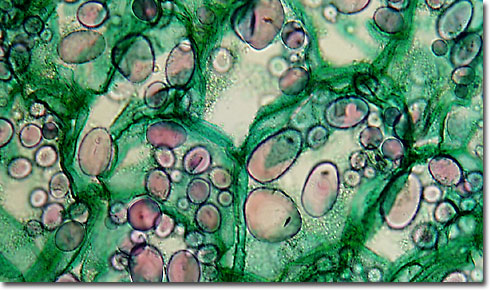
\includegraphics[width=0.8\textwidth]{3/figures/largepotato.jpg}
			\caption{Prueba de Figura}
			\label{fig1}
		\end{center}
		
	\end{figure}
	
	
	\section{Operacionalización de Variables}
	
	Nisi porta lorem mollis aliquam ut porttitor leo. Aenean pharetra magna ac placerat vestibulum. Est placerat in egestas erat imperdiet sed euismod. Velit euismod in pellentesque massa placerat. Enim praesent elementum facilisis leo vel fringilla. Ante in nibh mauris cursus mattis molestie a iaculis. Erat pellentesque adipiscing commodo elit at imperdiet dui accumsan sit. Porttitor lacus luctus accumsan tortor posuere ac ut. Tortor at auctor urna nunc id. A iaculis at erat pellentesque adipiscing commodo elit.
	\section{Instrumentos de medida}
	Nisi porta lorem mollis aliquam ut porttitor leo. Aenean pharetra magna ac placerat \begin{itemize}
		\item muscle and fat cells remove glucose from the blood,
		\item cells breakdown glucose via glycolysis and the citrate cycle, storing its energy in the form of ATP,
		\item liver and muscle store glucose as glycogen as a short-term energy reserve,
		\item adipose tissue stores glucose as fat for long-term energy reserve, and
		\item cells use glucose for protein synthesis.
	\end{itemize}
	
	\section{Técnicas de recolección de datos}
	Nisi porta lorem mollis aliquam ut porttitor leo. Aenean pharetra magna ac placerat vestibulum. Est placerat in egestas erat imperdiet sed euismod. Velit euismod in pellentesque massa placerat. Enim praesent elementum facilisis leo vel fringilla. Ante in nibh mauris cursus mattis molestie a iaculis. Erat pellentesque adipiscing commodo elit at imperdiet dui accumsan sit. Porttitor lacus luctus accumsan tortor posuere ac ut. Tortor at auctor urna nunc id. A iaculis at erat pellentesque adipiscing commodo elit.
	
	\LaTeX{} is great at typesetting mathematics. Let $X_1, X_2, \ldots, X_n$ be a sequence of independent and identically distributed random variables with
	\begin{equation}
		S_n = \frac{X_1 + X_2 + \cdots + X_n}{n}
		= \frac{1}{n}\sum_{i}^{n} X_i
		\label{eq1}
	\end{equation}
	
	La Ecuación \ref{eq1} denote their mean. Then as $n$ approaches infinity, the random variables $$\sqrt{n}(S_n - \mu)$$ converge in distribution to a normal $\mathcal{N}(0, \sigma^2)$.
	
	\section{Técnicas para el procesamiento y análisis de la información}
	Nisi porta lorem mollis aliquam ut porttitor leo. Aenean pharetra magna ac placerat vestibulum. Est placerat in egestas erat imperdiet sed euismod. Velit euismod in pellentesque massa placerat. Enim praesent elementum facilisis leo vel fringilla. Ante in nibh mauris cursus mattis molestie a iaculis. Erat pellentesque adipiscing commodo elit at imperdiet dui accumsan sit. Porttitor lacus luctus accumsan tortor posuere ac ut. Tortor at auctor urna nunc id. A iaculis at erat pellentesque adipiscing commodo elit.
	
	You can make lists with automatic numbering \dots
	
	\begin{enumerate}
		\item Like this,
		\item and like this.
	\end{enumerate}
	\dots or bullet points \dots
	\begin{itemize}
		\item Like this,
		\item and like this.
	\end{itemize}
	
	
	\section{Cronograma de actividades y presupuesto}
	Nisi porta lorem mollis aliquam ut porttitor leo. Aenean pharetra magna ac placerat vestibulum. Est placerat in egestas erat imperdiet sed euismod. Velit euismod in pellentesque massa placerat. Enim praesent elementum facilisis leo vel fringilla. Ante in nibh mauris cursus mattis molestie a iaculis. Erat pellentesque adipiscing commodo elit at imperdiet dui accumsan sit. Porttitor lacus luctus accumsan tortor posuere ac ut. Tortor at auctor urna nunc id. A iaculis at erat pellentesque adipiscing commodo elit.
	
	\begin{table}[h]
		
		
		\begin{tabular}{l|r}
			Item & Quantity \\\hline
			Widgets & 42 \\
			Gadgets & 13
		\end{tabular}
		\caption{\label{tab:widgets}An example table.}
	\end{table}
	
\end{comment}
